\chapter{IMPLEMENTATION}\thispagestyle{EmptyHeader}
\label{chp:2}
The drone is controlled by the user from the surface. The live feed from the drone is displayed to the used through the cable from the drone. The drone is made of of plastic material such as PVC pipes. The entire systems consist of two parts.

\section{Drone}

The drone is the major part of the proposed idea. This drone goes underwater and takes the live video from below surface. The drone consist of seven major parts such as

\begin{figure}[ht]
	\centering
	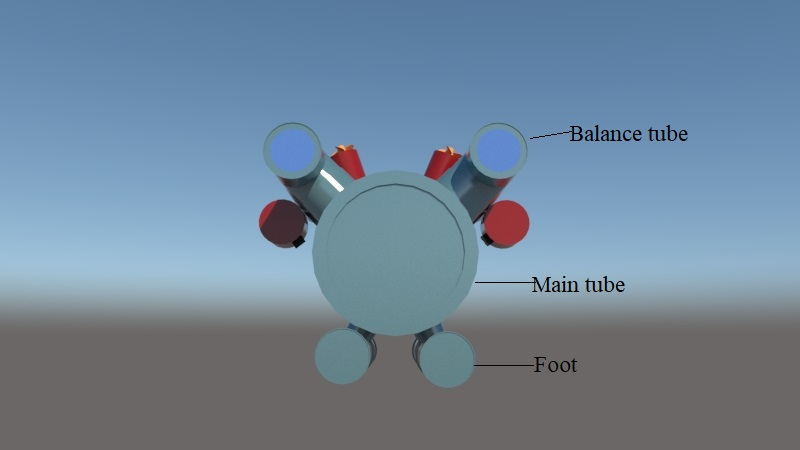
\includegraphics[width=\linewidth]{images/FrontView.jpg}
	\caption{Front View of Drone}
	\label{diag:sample}
\end{figure}

\begin{enumerate}
    \item Primary tube
    \item Balance tube
    \item Foot
    \item Vertical Propeller
    \item Horizontal Propeller
    \item Camera
    \item Led light
\end{enumerate}


The primary tube is the main structure of the drone. It consists of the battery and other important things such as microcontroller for controlling the propeller. The balance tube and the foot are directly connected to the principal tube. The LEDs are placed in the balance tube to give more quality to the video that is taken underwater. All the structures are air sealed so that water cannot penetrate into them. The foot and the balance tube are used as stabilizers for the primary tube. The navigation of the drone is controlled from the surface using the control unit. Arduino mega is used as the controller of this drone with 12V battery as its power supply. A 12Mp digital waterproof camera is used for video recording. 


\begin{figure}[ht]
	\centering
	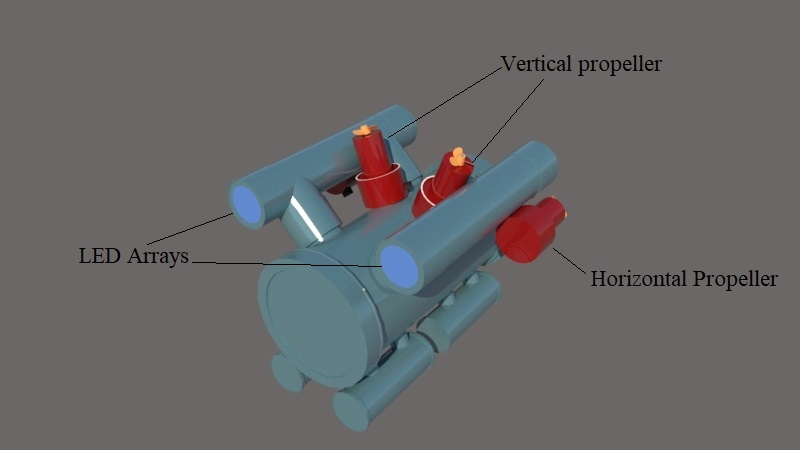
\includegraphics[width=\linewidth]{images/SideTop.jpg}
	\caption{Side View of Drone}
	\label{diag:sample}
\end{figure}

The live feed of the video is transmitted by USB cable from the camera to PC. The camera is also powered by the same 12V battery. Three dual H-Bridge LP298N Motor drivers are used to run the propellers and the LEDs. To maintain a constant voltage supply the motor driver is also used to control the LEDs. The motors used for the propellers are 12V DC boat bilge pump motors. These are underwater pumps which can also be used for the movement of the drone using the propellers. The figure 1 represents the front view of the drone and figure 2 shows the side view of the drone.

\section{Control Unit}
The control unit is the part which controls the drone from the surface. It has two joysticks to control to navigation of the drone. One joystick is used for the control of depth of drone underwater and other is used to control the forward and backward direction of the drone. The video feed is not included in the joystick it is done separately in the PC. The USB cable is responsible for the transmission of video from drone to PC. The LEDs present in the drone is also controlled by the control unit. 
The block diagram of the drone and control unit is shown in figure 3.

\begin{figure}[ht]
	\centering
	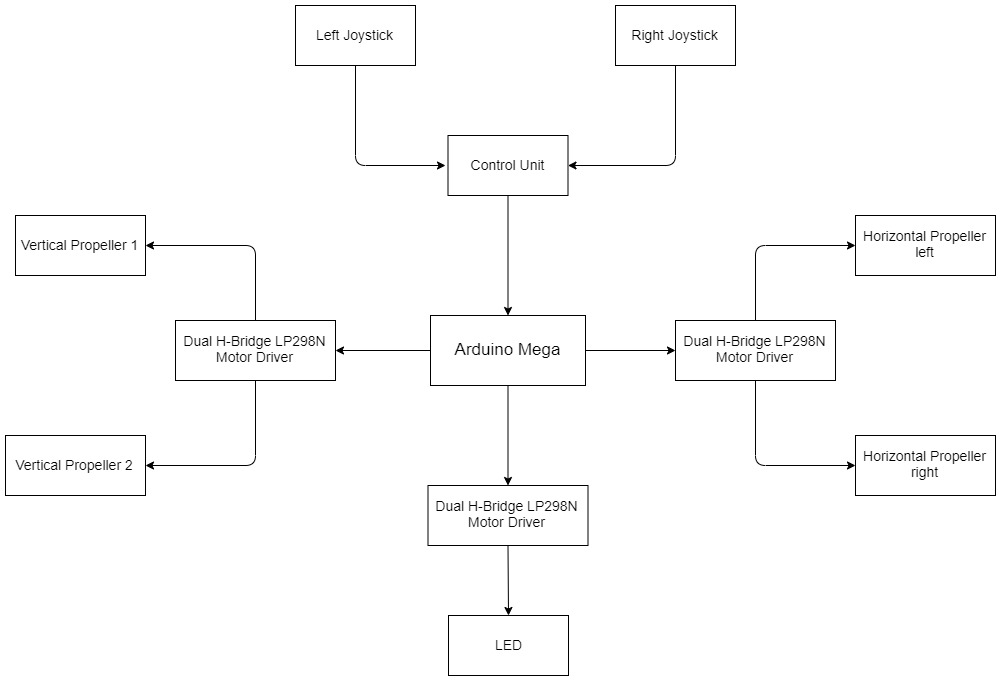
\includegraphics[width=\linewidth]{images/BlockDiagram.jpg}
	\caption{Block Diagram}
	\label{diag:sample}
\end{figure}